\section{Criteria to begin the LSST}

Armed with an understanding of the system performance as outlined above and the Operations team readiness, we will use a set of objective criteria to gate the start of the LSST. These criteria will be concise and easily understandable so that the community of scientists and stakeholders counting on Rubin and the survey will have confidence the Observatory is on track.

The criteria we will use that are listed below are only to start the survey. There may be key processes within the overall system, including data management and processing that require further work after handover (beyond the construction project requirements), but unless they would prevent delaying the survey start, they are not discussed or enumerated here.

The Operations team discussed an initial set of criteria with the Science Advisory Committee and community at the 2024 Rubin Community Workshop. The current criteria have been evolved since that meeting and are shown in the table below.

\begin{table}[]
\renewcommand{\arraystretch}{2}
\small
\centering
\caption{Survey Start Criteria}\label{tab:criteria}
\begin{tabular}{|p{0.25in}|p{1in}|p{4in}|p{1.0in}|}
\hline
Item & Criterion & Description& Status \\
\hline \hline

1 & \makecell[l]{LSSTCam\\ Maintenance} & Before the completion of SV, it is understood whether or not off TMA Camera maintenance will be needed within the first year of Operations.& No off TMA maintenance required.  \\\hline  

2 & SRD &All science requirements that can be verified with SV data are verified or expected to be verified within 3 months of completion of SV. & Status at CCR3 \\\hline

3 & Dome & The dome environment is not limiting typical performance. &\makecell[l]{ Not controlled \\until after \\Handover} \\\hline

4 & Calibration & All necessary calibration data products are available at the time any LSST data are obtained or can be obtained after the fact without invalidating the observed data for inclusion in the LSST. & Status at CCR3 \\\hline

5& DIQ& Delivered Image quality contribution of system is better than or equal to 0.4$\arcsec$ & \makecell[l]{Currently 0.6$\arcsec$ \\system \\contribution}\\\hline

6 & Normalized \'{E}tendue & Survey speed  is $>$ 0.7. & Currently 0.68 \\\hline

7 & Cadence & The first six months of survey schedule as expected to be executed includes details of the system as currently performing.& In progress\\\hline

8 & Early Science&DP2 observations are completed as planned \citep{RTN-011}.& Status at CCR3 \\

\hline
\end{tabular}
\end{table}

These criteria are not comprehensive with respect to LSST success. They are intended only to guide the confident commencement of the survey. The initial boundary condition is a successful completion of the construction project. This means the construction completeness reviews have been successfully completed and NSF and DOE have accepted the system as the one they intended to build.

The criteria cover a range of contexts. Most look to be well in hand based on what we know about commissioning progress and what has been reported at CCR2/ORR1. Item 1 is already met. We do not expect to have to remove the camera for maintenance before we begin the survey. Item 2 is needed to ensure some key aspects of the system don't need verification before we embark on the LSST. Some long term SRD requirements need a significant amount of data to finally validate. But we can be assured data being taken are going to be valid for the LSST if the requirements that can be validated with SV data have been. This will be confirmed at CCR3. The calibration system (item 4)  is in the advanced stages of validation. By CCR3, we can be assured no outstanding calibration needs will limit the taking of images for the LSST. For item 7, we are already folding in as delivered performance into the survey simulations. We can be confident the remaining performance status can be adapted into the initial LSST cadence by the time we are ready to start. Once SV data taking is complete, we will know the content of DP2 (item 8) and be able to decide whether or not any augmentation is critical for community preparation before data release 1 \citep[DR1; see][]{RTN-011}. 

This leaves the "big 3," the dome environment, system contribution to DIQ, and Normalized \'{E}tendue. These are discussed next in more detail.

\subsection{Dome Environmental Control}
The dome is the last major subsystem to be completed. Indeed it will not be done until mid 2026. The critical aspects that are needed are to install, provide control for, and optimize the actuators for the dome louvers. There are 40 louvers, and some large fraction need to be operable (open at fractions consistent with telemetry in real time for temperatures and wind). The first actuators are installed now and may be operable before the shutdown. Still more will need to be brought on line after the handover. If the louvers limit us to worse than typical min SRD performance, we won't be able to start the LSST until they are largely deployed and in routine operation. 

There are large ducts that will provide for air distribution via the main air handlers inside the facility. This system should improve our ability to maintain the enclosure at closer to the required nighttime temperature during the day time. Hitting the right temperature in the environment around the telescope is critical to good IQ during the night. The ducts are necessary but not sufficient. We will also need to gain experience in forecasting the coming night's temperature to be able to use the air conditioning effectively (i.e. to set the system to hit the right target). 

Further use of available temperature sensors on the telescope and in the dome will help on going analyses aimed at improving the AOS and thermal control of the optics in real time. 

The total contribution to DIQ from the dome environment is modest. Including all sources of turbulence generated by the facility, the budget to contribute to the DIQ is only 0.09$\arcsec$. Clearly all systems for controlling these contributions need to be working well and reliably. The observatory will need to rely on the ability to characterize parts of the DIQ coming from this environment. Thus we will prioritize reliable operation and calibration of our DIMM, in-dome seeing monitors, as well as the atmospheric profiler on Cerro Pach\'{on}, RINGSS.  

\subsection{Normalized \'{E}tendue}
Much of the effective speed (Normalized  \'{E}tendue) is already demonstrated to be sufficient to start the LSST, The field of view factor, fA, is excellent and stable. The sensitivity factor, fS, is also very good. This factor has the potential to help overall performance because of its dependence on delivered image quality. Getting the system contribution from 0.6 to 0.4 (coupled with site atmospheric seeing of 0.7$\arcsec$) would raise fS from 0.94 to 1.3. Apart from this, all the optics are delivered as is the focal plane. The performance of all these components is excellent and can be maintained. The observing efficiency or fO is also in good shape. The telescope dynamic performance (slew speed, acceleration, and jerk) is sufficient for the LSST planned cadence. 

The TMA currently can move faster than we operate it due to the need to improve the control of dynamic loads on the glass via force actuators. However the current performance with glass is captured in the scheduler simulator and is only a modest hit to LSST. We will continue to work on improved dynamic control even as we operate for LSST. Slew and settle performance are well understood and adequate. Modest gains on fO are forecast for the rest of SV and early operations. We expect the current value to go from 0.97 to 1.05. 

This leaves the System Availability, Current performance of 0.75 needs to be improved. Doing only science like observations we have reached 85$\%$ at times. We need to continue to improve on procedures and reliability of systems throughout the summit facility as we go forward. This means training for faster troubleshooting and fault recovery, making communications on the telescope system bus more reliable, improving reliability of telescope, dome, and camera functions. These have all seen marked progress as expected though out system integration, test, and commissioning. We will assume current performance of 75$\%$ conservatively. 

The minimum Normalized \'{E}tendue is 0.7$\arcsec$ in the SRD. This level is nearly in hand; see Table~\ref{tab:factors} and the "Sustained Performance values." We will start the LSST consistent with System Availability of 75$\%$ which leads to fE $=$ 1.01 using the Demonstrated Capability column f factors in Table~\ref{tab:factors}. However, the actual value will be better given that we expect the System Availability to improve significantly. 

\subsection{DIQ}

The single most important gain needed to get to the LSST start is clearly the typical DIQ. We will not start the LSST until this sustained performance reflects a system contribution of $\le$ 0.4$\arcsec$, the minimum SRD requirement. The very best the system contribution can be given current as build measurements is 0.327$\arcsec$. 

Improving the system contribution to the DIQ requires continued effort on the control of optics and the dome environment. Putting this together with the criteria above results in the region of the performance diagram we can use to gate starting the LSST as depicted in Figure~\ref{speed3}. The survey can begin once the system contribution to DIQ is 0.4$\arcsec$ or less and the effective survey speed is 1.01 or better (see Table~\ref{tab:factors} and assume System Availability is 75$\%$).

\begin{figure}[t]
  \centering
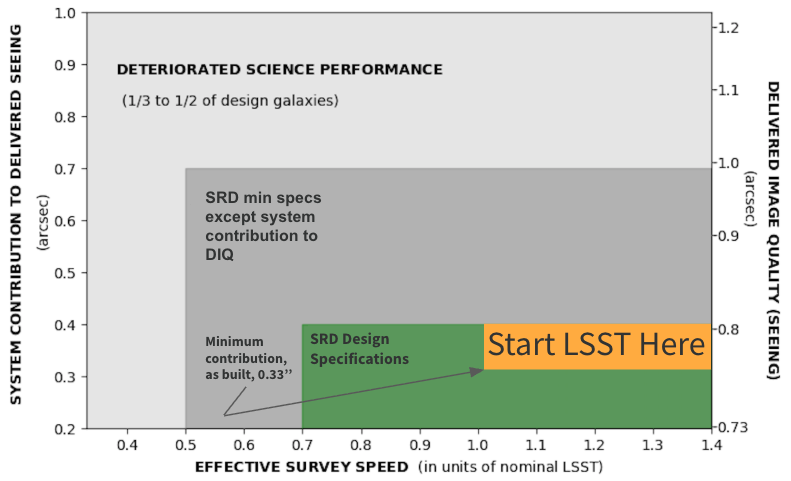
\includegraphics[width=0.85\linewidth]{speed3.png}
\caption{Image quality versus effective survey speed or Normalized \'{E}tendue. The large orange rectangle represents the region in this space within which we can confidently start the LSST.}
\label{speed3}
\end{figure}

\newpage
